{\section{Wyniki i analiza pomiarów}}

\subsection{Pomiar rezystancji w układzie dwupunktowym omomierzem AGILENT} % ZADANIE 1,2

\begin{figure}[!h]
    \centering
    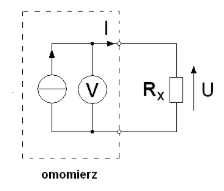
\includegraphics[width = 70mm]{imgs/schamat1_cw3.png}
    \caption{Schemat pomiarowy układu dwupunktowego}
    \label{fig:enter-label}
\end{figure}

\newpage
W tabelach poniżej zostały zapisane odczytane oraz zmierzone wartości rezystancji.

\begin{table}[!h]
    \centering
    \begin{tabular}{|c|c|c||c|c|c|}\hline
        Nazwa                             & R            & Tolerancja           & $R_{zm}$         & Zakres      & Niepewność \\ \hline
      \multirow{3}{*}{Opornik Wzorcowy}   & $10k\Omega$  & 0,03\%               & $9,9994k\Omega$  & $10k\Omega$ & $(9,9994 \pm 0,0012)k\Omega$ \\ 
                                          & $10\Omega$   & 0,01\%               & $10,077\Omega$   & $100\Omega$ & $(10,077 \pm 0,005)\Omega$  \\ 
                                          & $1\Omega$    & 0,01\%               & $1,073\Omega$    & $100\Omega$ & $(1,073 \pm 0,004)\Omega$  \\ \hline
      \multirow{3}{*}{Rezystor zwykły}    & $220k\Omega$ & \multirow{3}{*}{5\%} & $0,22129M\Omega$ & $1M\Omega$  & $(0,22129 \pm 0,00003)M\Omega$ \\
                                          & $6,8k\Omega$ &                      & $6,77448k\Omega$ & $10k\Omega$ & $(6,77448 \pm 0,00078)k\Omega$ \\
                                          & $100\Omega$  &                      & $99,404\Omega$   & $100\Omega$ & $(99,404 \pm 0,0014)\Omega$ \\ \hline
                            Rezystor mocy & $2,2\Omega$  & 1\%                  & $2,297\Omega$    & $100\Omega$ & $(2,297 \pm 0,004)\Omega$ \\ \hline
    \end{tabular}
    \caption{Wartości odczytane wraz z wartościami zmierzonymi oraz niepewnościami}
    \label{tab:my_label}
\end{table}

\subsection{Pomiar rezystancji rezystorów na płytce omomierzem analogowym} % ZADANIE 3
%==================
\begin{table}[!h]
    \centering
    \begin{tabular}{|c|c|c|c|}\hline
        Rezystancja & Zakres & Pomiar & Niepewność \\ \hline
         $220k\Omega$ & x$1k\Omega$ & pomiar nieczytelny & pomiar nieczytelny  \\ \hline
         $6,8k\Omega$ & x$1k\Omega$ & $5,75k\Omega$ &  $(5,75 \pm 50)k\Omega$ \\ \hline
         $100\Omega$  & x$10\Omega$ & $110\Omega$ &  $(110 \pm 500)\Omega$\\ \hline
    \end{tabular}
    \caption{Caption}
    \label{tab:my_label}
\end{table}
%================ wnioskiem do tej tabeli jest to że na multimetrze analogowym ciężko jest odczytać dokładnie rezystancję
\subsection{Pomiar rezystorów wzorcowych omomierzem AGILENT w układzie czteropunktowym} % ZADANIE 4,14

\begin{figure}[!h]
    \centering
    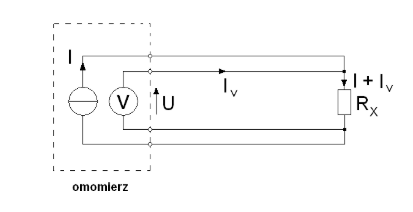
\includegraphics{imgs/schamat2_cw3.png}
    \caption{Schemat pomiarowy układu czteropunktowego}
    \label{fig:enter-label}
\end{figure}
%===================== TABELKA Z POMIARAMI PLUS NIEPEWNOŚĆ 

\begin{table}[!h]
    \centering
    \begin{tabular}{|c|c|c|c|c|}
        \hline
        Rezystancja & Tolerancja & Pomiar          & Zakres      & Niepewność \\ \hline
        $1\Omega$   & 0,01\%     & $1,000\Omega$   & $100\Omega$ & $(1,000 \pm 0,004)\Omega$\\ \hline
        $10\Omega$  & 0,01\%     & $10,000\Omega$  & $100\Omega$ & $(10,000 \pm 0,005)\Omega$\\ \hline 
        $10k\Omega$ & 0,03\%     & $9,9993k\Omega$ & $10k\Omega$ & $(9,9993 \pm 0,0011)k\Omega$ \\ \hline 
    \end{tabular}
    \caption{Caption}
    \label{tab:tabela-nr4}
\end{table}

\newpage
{\subsection{Pomiar rezystancji rezystora mocy za pomocą przewodów o różnych właściwościach i omomierza AGILENT w układzie dwupunktowym i czteropunktowym}} % ZADANIE 5,6,7

\begin{table}[!h]
    \centering
    \begin{tabular}{|c|c|c|c|}\hline
        Pomiar & Zakres & Rodzaj przewodów \\ \hline
        $2,416\Omega$ & $100\Omega$ & cienkie 1m \\ \hline
        $2,374\Omega$ & $100\Omega$ & grube 1m \\ \hline
        $2,293\Omega$ & $100\Omega$ & grube 20cm \\ \hline
    \end{tabular}
    \caption{Wartości zmierzone w układzie dwupunktowym}
    \label{tab:tabela-nr5}
\end{table}

\indent Po dokonaniu pomiarów rezystora została zmierzona rezystancja przewodów pomiarowych:

\begin{table}[!h]
    \centering
    \begin{tabular}{|c|c|c|} \hline
        Pomiar        & Zakres      & Rodzaj przewodów \\ \hline
        $0,200\Omega$ & $100\Omega$ & cienkie 1m \\ \hline
        $0,149\Omega$ & $100\Omega$ & grube 1m \\ \hline
        $0,047\Omega$ & $100\Omega$ & grube 20cm \\ \hline
    \end{tabular}
    \caption{Rezystancja przewodów użytych do pomiaru w układzie dwupunktowym}
    \label{tab:tabela-nr6}
\end{table}

%=================== rezystancja przewodów bez tabeli ===================
Po dokonaniu obu pomiarów możemy obliczyć właściwą wartość oporu rezystorów. $ R = R_{zm}-R_{przewodu}$
\begin{itemize}
    \item Przewód cienki 1m - $R = 2,416\Omega - 0,200\Omega = 2,216\Omega$
    \item Przewód gruby 1m - $R = 2,374\Omega - 0,149\Omega = 2,225\Omega$
    \item Przewód gruby 20cm - $R = 2,293\Omega - 0,047\Omega = 2,246\Omega$
\end{itemize}
%=================== ############################### ====================

Po zmierzeniu oporu rezystora mocy o nominalnej wartości $2,2\Omega$ w układzie czteropunktowym wynik pomiaru to $2,233\Omega$ (na zakresie $100\Omega$).
Można zauważyć, że wynik pomiary z użyciem układu czteropnuktowego jest bliski rezystancji otrzymanej po dokonaniu dwóch osobnych pomiarów w układzie dwupunktowym i obliczeniu różnicy owych pomiarów.
Wychodzi na to, że metoda z użyciem układu czteropunktowego jest szybsza i tak samo dokładna.

\subsection{Oszacowanie maksymalnego napięcia dla rezystorów} % ZADANIE 8 I 9

Aby oszacować wartość maksymalnego napięcia które możemy przyłożyć do rezystora mocy tak aby nie przekroczyć 50W dla rezystora mocy oraz 2W dla reszty rezystorów musimy skorzystać ze wzoru poniżej:

$$P=\frac{U^2}{R} \hspace{1cm} P=I^2 \cdot R$$

Po przekształceniu:

$$U=\sqrt{P \cdot R} \hspace{1cm} I=\sqrt{\frac{P}{R}}$$

%================= Tabela z wynikami ===================
\begin{table}[!h]
    \centering
    \begin{tabular}{|c|c|c|c|}\hline
        Rezystancja & $P_{Max}$ & $U_{Max}$ & $I_{Max}$\\ \hline
       Rezystor mocy $2,2\Omega$  & 50W & 10,49V & 4,77A \\ \hline
        $220k\Omega$ & \multirow{3}{*}{2W} & 663,33V & 0,003A \\ 
        $6,8k\Omega$ &  & 116,62V & 0,017A \\ 
        $100\Omega$ &  & 14,14V & 0,14A \\ \hline
    \end{tabular}
    \caption{Maksymalne napięcie i prąd}
    \label{tab:my_label}
\end{table}
%===========================================================

\newpage
\subsection{Pomiar rezystancji w układzie poprawnego pomiaru napięcia i prądu} % ZADANIE 10,11,12,13,15
\subsubsection{Poprawny pomiar napięcia}

\begin{figure}[!h]
    \centering
    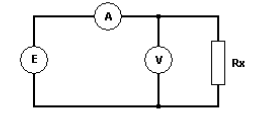
\includegraphics{imgs/schamat3_cw3.png}
    \caption{Układ poprawnego pomiaru napięcia}
    \label{fig:enter-label}
\end{figure}

\begin{table}[!ht]
    \centering
    \begin{tabular}{|c||c|c|c|c|c|c|} \hline
        Rezystancja                   & Pomiar   & Zakres & Obliczona rezystancja             & Niepewność & Błąd bezwzględny & Błąd względny \\ \hline
        \multirow{2}{*}{$2,2\Omega$}  & 1,8222A  & 3A     & \multirow{2}{*}{$2,243\Omega$}    & \multirow{2}{*}{$\pm 0,003$} &\multirow{2}{*}{$\pm 0,0000005\Omega$} & \multirow{2}{*}{$0,00002\%$}\\
                                      & 4,0867V  & 10V    &                                   & & & \\ \hline
        \multirow{2}{*}{$220k\Omega$} & 0,0238mA & 10mA   & \multirow{2}{*}{$213,722k\Omega$} & \multirow{2}{*}{$\pm 18066,75$} &\multirow{2}{*}{$\pm 4668\Omega$} & \multirow{2}{*}{$2,14\%$}\\
                                      & 5,0866V  & 10V    &                                   & & & \\ \hline
        \multirow{2}{*}{$6,8k\Omega$} & 6,7543mA & 10mA   & \multirow{2}{*}{$752,558\Omega$}  & \multirow{2}{*}{$\pm 0,64$} &\multirow{2}{*}{$\pm 0,062\Omega$} & \multirow{2}{*}{$0,008\%$} \\
                                      & 5,0830V  & 10V    &                                   & & & \\ \hline
        \multirow{2}{*}{$100\Omega$}  & 48,553mA & 10mA   & \multirow{2}{*}{$99,254\Omega$}   & \multirow{2}{*}{$\pm 0,06$} &\multirow{2}{*}{$\pm 0,001\Omega$} & \multirow{2}{*}{$0,001\%$}\\
                                      & 4,8191V  & 10V    &                                   & & & \\ \hline
    \end{tabular}
    \caption{Tabela pomiarów dla poprawnego pomiaru napięcia}
    \label{tab:my_label}
\end{table}

\subsubsection{Poprawny pomiar natężenia prądu}

\begin{figure}[!h]
    \centering
    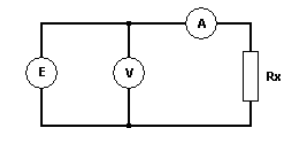
\includegraphics{imgs/schamat4_cw3.png}
    \caption{Układ poprawnego pomiaru prądu}
    \label{fig:enter-label}
\end{figure}

\begin{table}[!ht]
    \centering
    \begin{tabular}{|c||c|c|c|c|c|c|} \hline
        Rezystancja                   & Pomiar   & Zakres & Obliczona rezystancja             & Niepewność                            & Błąd bezwzględny & Błąd względny \\ \hline
        \multirow{2}{*}{$2,2\Omega$}  & 1,8293A  & 3A     & \multirow{2}{*}{$2,744\Omega$}    & \multirow{2}{*}{$\pm 0,00157\Omega$}  & \multirow{2}{*}{$\pm 5\Omega$} & \multirow{2}{*}{182,24\%}\\
                                      & 5,0329V  & 10V    &                                   &                                       & & \\ \hline
        \multirow{2}{*}{$220k\Omega$} & 0,0230mA & 10mA   & \multirow{2}{*}{$221,154k\Omega$} & \multirow{2}{*}{$\pm 2,193k\Omega$}   & \multirow{2}{*}{$\pm 0,1\Omega$} & \multirow{2}{*}{0,045\%}\\
                                      & 5,0866V  & 10V    &                                   &                                       &  & \\ \hline
        \multirow{2}{*}{$6,8k\Omega$} & 6,7538mA & 10mA   & \multirow{2}{*}{$752,556\Omega$}  & \multirow{2}{*}{$\pm 0,00553\Omega$}  & \multirow{2}{*}{$\pm 0,1\Omega$} & \multirow{2}{*}{0,013\%}\\
                                      & 5,0871V  & 10V    &                                   &                                       & & \\ \hline
        \multirow{2}{*}{$100\Omega$}  & 48,570mA & 10mA   & \multirow{2}{*}{$104,658\Omega$}  & \multirow{2}{*}{$\pm 0,000510\Omega$} & \multirow{2}{*}{$\pm 0,1\Omega$} & \multirow{2}{*}{0,096\%}\\
                                      & 5,0857V  & 10V    &                                   &                                       & & \\ \hline
    \end{tabular}
    \caption{Tabela pomiarów dla poprawnego pomiaru natężenia prądu}
    \label{tab:my_label}
\end{table}

\newpage
Aby obliczyć błędy pomiarowe tych metod zostały wykorzystane następujące wzory:

\begin{equation*}
    u(R_{zm})=\sqrt{\left(\frac{1}{I_A}*u(U_V)\right)^2+\left(\frac{-U_V}{(I_A)^2}*u(I_A)\right)^2}
\end{equation*}

Gdzie:
\begin{itemize}
    \item $u(U_{zm})$ - Niepewność z prawa propagacji
    \item $I_A$ - prąd zmierzony
    \item $u(U_V)$ - niepewność pomiaru napięcia
    \item $U_V$ - napięcie zmierzone
    \item $u(I_A)$ - niepewność pomiaru prądu
\end{itemize}

\vspace{0.4cm}
Błąd systematyczny bezwzględny $\Delta R_s$
\begin{equation*}
    \Delta R_S=\frac{R_x \cdot R_v}{R_x + R_v}-R_x
\end{equation*}

Gdzie:
\begin{itemize}
    \item $R_x$ - Rezystancja zmierzona
    \item $R_v$ -  rezystancja woltomierza
\end{itemize}

Względny błąd systematyczny to:
\begin{equation*}
    \delta R_s=\frac{-R_x}{R_x+R_v} \cdot 100\%
\end{equation*}

\vspace{0.5cm}
Następnie została obliczona rezystancja graniczna dla dwóch pierwszych i ostatnich zakresów dostępnych na multimetrze Agilent. Wykorzystaliśmy do tego następujący wzór:

$$R_{gr}=\sqrt{R_A \cdot R_V}$$

Gdzie:
\begin{itemize}
    \item $R_A$ - Rezystancja wewnętrzna amperomierza
    \item $R_V$ - Rezystancja wewnętrzna woltomierza
\end{itemize}

\vspace{0.2cm}
Poniżej zostały przedstawione wyniki obliczeń:
\begin{enumerate}
    \item Dla zakresu $100M\Omega$ i $10M\Omega$ - $R_{gr}\approx 7,1k\Omega$
    \item Dla zakresu $100\Omega$ i $1k\Omega$ - $R_{gr}\approx 1k\Omega$
\end{enumerate}